The functionality of the FPGA timetagger is primarily accessed through
two graphical interfaces provided by {\tt timetag\_tools}: {\tt
 timetag\_ui} and {\tt timetag\_seq\_ui}. These are both installed in
the system application list as shown in \ref{Fig:Dash}.

\section{Timetagger UI}

The timetagger interface, {\tt timetag\_ui}, is a graphical frontend to
the device's timetagging functionality. The main window is shown in Figure 
\ref{Fig:MainWindow}.

\begin{figure}
  \center
  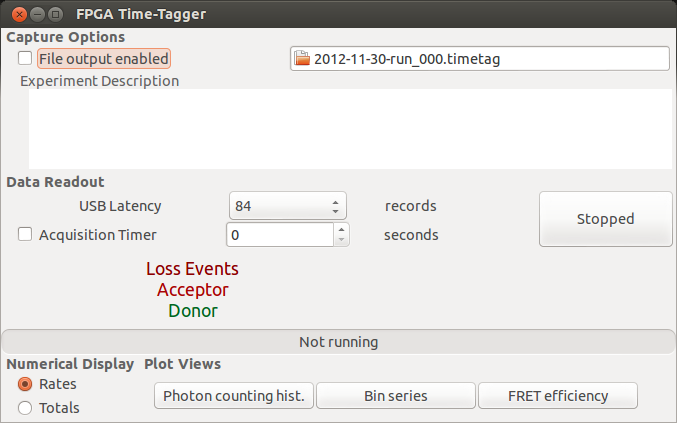
\includegraphics[scale=0.5]{timetag-window.png}
  \caption{The main window of {\tt timetag\_ui}.}
  \label{Fig:MainWindow}
\end{figure}

The first time the interface is started it will likely be necessary to
look over the channel configuration. This is acheived through the
``Edit channel configuration...'' entry in the ``File'' menu. This
will display the dialog box shown in Figure
\ref{Fig:ChannelConfig}. Here one can enable and disable acquisition
on individual channels, as well as choose descriptive labels and colors
for each. These settings are stored in a configuration file in the
user's home directory.

\begin{figure}
  \center
  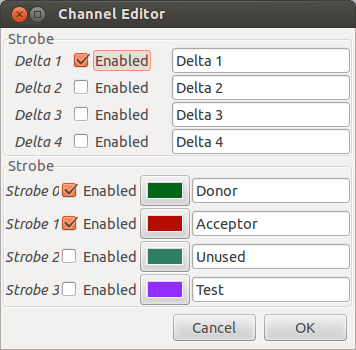
\includegraphics[scale=0.5]{channel-editor.png}
  \caption{The channel configuration window of {\tt timetag\_ui}.}
  \label{Fig:ChannelConfig}
\end{figure}

To begin data acquisition, simply enter a file name, ensure that file
output is enabled by checking the box bearing the label ``File output
enabled,'' and press the button labelled ``Stopped''. Additionally one
can enter an experiment description to be saved alongside the data and
optionally set a time after which acquisition will be stopped.

After beginning data acquisition, the instantaneous count rates will
be shown next to their respective channel names. Alternatively, one
can view the total event count by selecting the ``Totals'' radio
button in the lower left corner of the window.

In addition to these numerical indicators, {\tt timetag\_ui} provides
several plot views available through the buttons on the lower right
corner of the main window. Moreover, each of these windows have a
variety of configuration options available by clicking on the small
triangle on the lower left hand corner.

The photon counting histogram shows a histogram of the number of
photon arrivals to occur in a given bin time (configurable as the
``Bin Time'') for each channel. The size of the histogram bins is
configured with the ``Histogram bin width'' setting.

\begin{figure}
  \center
  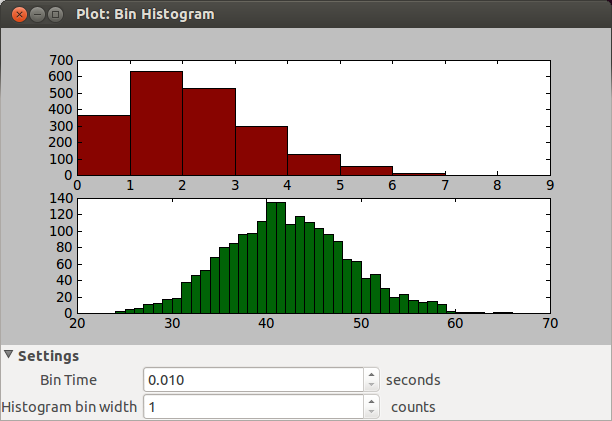
\includegraphics[scale=0.5]{count-hist.png}
  \caption{The photon count histogram view}
  \label{Fig:CountHist}
\end{figure}

The bin series view shows a time series of the binned events. The bin
width and total plotted duration is configurable, as is the Y axis
range.

\begin{figure}
  \center
  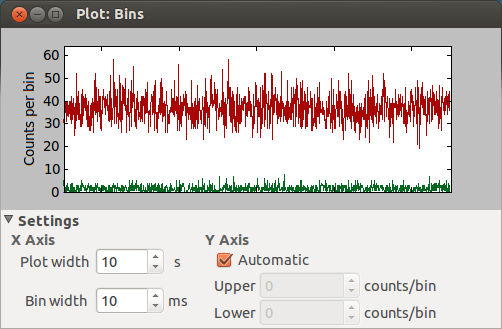
\includegraphics[scale=0.5]{bin-series.png}
  \caption{The bin series view}
  \label{Fig:BinSeries}
\end{figure}

The FRET histogram view offers a convenient way to visualize the state
of an on-going FRET experiment with a simple binning/threshold
analysis. Here the acceptor and donor channels are configurable, as
well as the bin time, threshold, and number of histogram bins. Note
that this is an extremely simple analysis which makes no attempt at
correcting for common experiment artifacts such as crosstalk and
$\gamma$ parameter.

\begin{figure}
  \center
  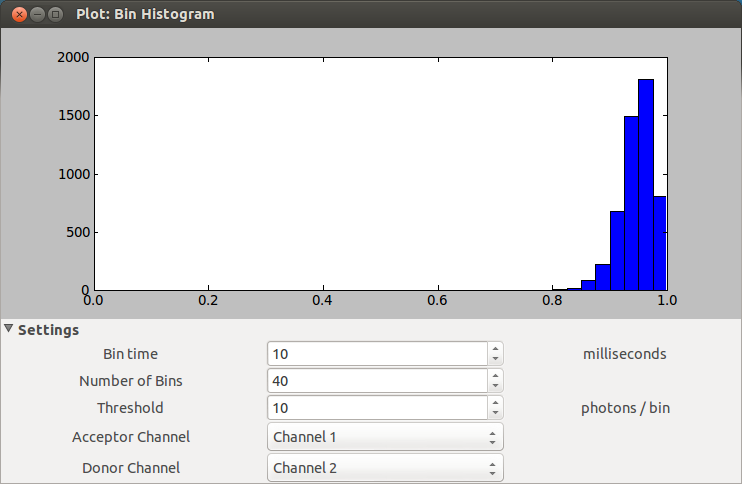
\includegraphics[scale=0.5]{fret-hist.png}
  \caption{The FRET histogram view}
  \label{Fig:FretHist}
\end{figure}


\section{Analysis}

While the {\tt timetag\_ui} provides some simple views for quickly
visualizing the state of an on-going experiment, these are not
intended to replace proper data analysis. For analysis of timetag data
we provide a suite of tools in the {\tt photon\_tools}
package. Installation of these tools has been discussed in
\ref{Sec:InstallingPhotonTools} and further documentation is provided
with the package.
